\selectlanguage{english}%

\chapter{Implementação} \label{capImp}

A implementação do modelo na bancada inicia-se com sua identificação

\section{Identificação}

\begin{figure}[H]
	\centering
	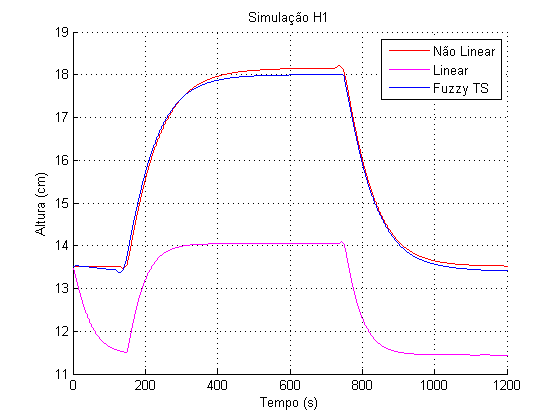
\includegraphics[width=0.7\textwidth]{img/FM_h1_5_10_15.png}
	\caption{Imagem Identificação - Modelo 1}
	\label{figH1TS2}
\end{figure}

\begin{figure}[H]
	\centering
	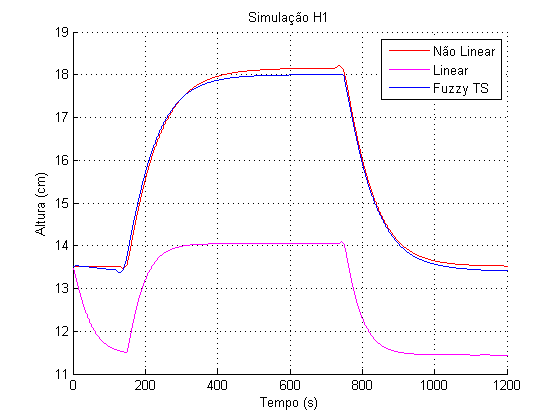
\includegraphics[width=0.7\textwidth]{img/FM_h1_5_10_15.png}
	\caption{Imagem Identificação - Modelo 2}
	\label{figH1TS2}
\end{figure}

\begin{figure}[H]
	\centering
	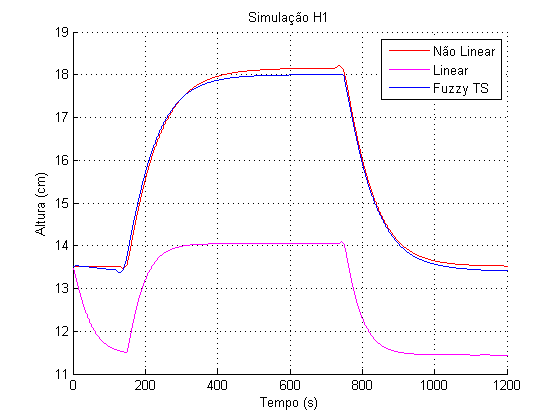
\includegraphics[width=0.7\textwidth]{img/FM_h1_5_10_15.png}
	\caption{Imagem Identificação - Modelo 3}
	\label{figH1TS2}
\end{figure}

\begin{figure}[H]
	\centering
	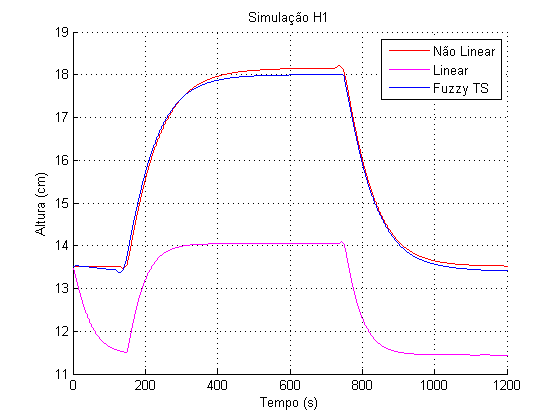
\includegraphics[width=0.7\textwidth]{img/FM_h1_5_10_15.png}
	\caption{Imagem Identificação - Modelo 4}
	\label{figH1TS2}
\end{figure}

\begin{figure}[H]
	\centering
	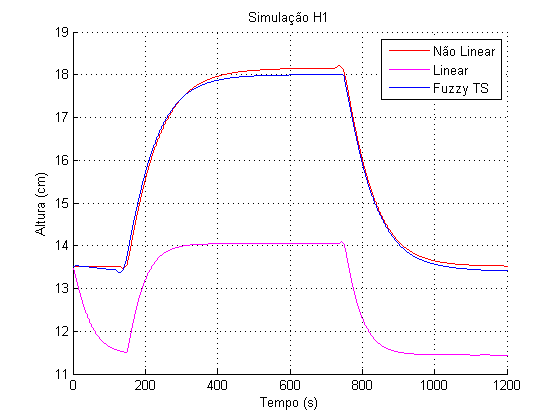
\includegraphics[width=0.7\textwidth]{img/FM_h1_5_10_15.png}
	\caption{Imagem Identificação - Comparação Modelo Fuzzy}
	\label{figH1TS2}
\end{figure}

\section{CLP}

\begin{figure}[H]
	\centering
	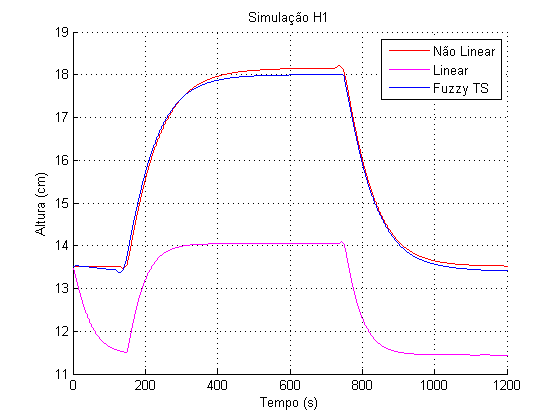
\includegraphics[width=0.7\textwidth]{img/FM_h1_5_10_15.png}
	\caption{Texto Estruturado}
	\label{figH1TS2}
\end{figure}

\begin{figure}[H]
	\centering
	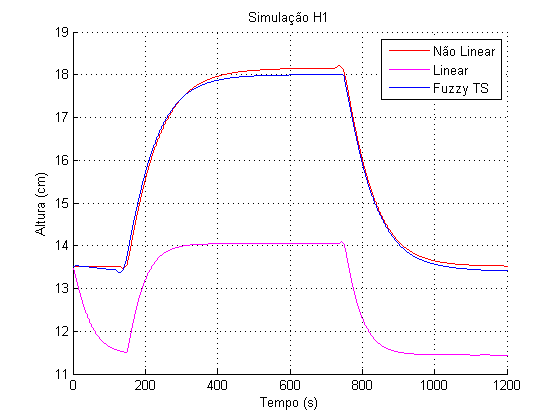
\includegraphics[width=0.7\textwidth]{img/FM_h1_5_10_15.png}
	\caption{Diagrama de Blocos}
	\label{figH1TS2}
\end{figure}

\selectlanguage{brazil}%

